% Options for packages loaded elsewhere
\PassOptionsToPackage{unicode}{hyperref}
\PassOptionsToPackage{hyphens}{url}
%
\documentclass[
]{article}
\usepackage{lmodern}
\usepackage{amssymb,amsmath}
\usepackage{ifxetex,ifluatex}
\ifnum 0\ifxetex 1\fi\ifluatex 1\fi=0 % if pdftex
  \usepackage[T1]{fontenc}
  \usepackage[utf8]{inputenc}
  \usepackage{textcomp} % provide euro and other symbols
\else % if luatex or xetex
  \usepackage{unicode-math}
  \defaultfontfeatures{Scale=MatchLowercase}
  \defaultfontfeatures[\rmfamily]{Ligatures=TeX,Scale=1}
\fi
% Use upquote if available, for straight quotes in verbatim environments
\IfFileExists{upquote.sty}{\usepackage{upquote}}{}
\IfFileExists{microtype.sty}{% use microtype if available
  \usepackage[]{microtype}
  \UseMicrotypeSet[protrusion]{basicmath} % disable protrusion for tt fonts
}{}
\makeatletter
\@ifundefined{KOMAClassName}{% if non-KOMA class
  \IfFileExists{parskip.sty}{%
    \usepackage{parskip}
  }{% else
    \setlength{\parindent}{0pt}
    \setlength{\parskip}{6pt plus 2pt minus 1pt}}
}{% if KOMA class
  \KOMAoptions{parskip=half}}
\makeatother
\usepackage{xcolor}
\IfFileExists{xurl.sty}{\usepackage{xurl}}{} % add URL line breaks if available
\IfFileExists{bookmark.sty}{\usepackage{bookmark}}{\usepackage{hyperref}}
\hypersetup{
  pdftitle={Lasma dataset},
  hidelinks,
  pdfcreator={LaTeX via pandoc}}
\urlstyle{same} % disable monospaced font for URLs
\usepackage[margin=1in]{geometry}
\usepackage{color}
\usepackage{fancyvrb}
\newcommand{\VerbBar}{|}
\newcommand{\VERB}{\Verb[commandchars=\\\{\}]}
\DefineVerbatimEnvironment{Highlighting}{Verbatim}{commandchars=\\\{\}}
% Add ',fontsize=\small' for more characters per line
\usepackage{framed}
\definecolor{shadecolor}{RGB}{248,248,248}
\newenvironment{Shaded}{\begin{snugshade}}{\end{snugshade}}
\newcommand{\AlertTok}[1]{\textcolor[rgb]{0.94,0.16,0.16}{#1}}
\newcommand{\AnnotationTok}[1]{\textcolor[rgb]{0.56,0.35,0.01}{\textbf{\textit{#1}}}}
\newcommand{\AttributeTok}[1]{\textcolor[rgb]{0.77,0.63,0.00}{#1}}
\newcommand{\BaseNTok}[1]{\textcolor[rgb]{0.00,0.00,0.81}{#1}}
\newcommand{\BuiltInTok}[1]{#1}
\newcommand{\CharTok}[1]{\textcolor[rgb]{0.31,0.60,0.02}{#1}}
\newcommand{\CommentTok}[1]{\textcolor[rgb]{0.56,0.35,0.01}{\textit{#1}}}
\newcommand{\CommentVarTok}[1]{\textcolor[rgb]{0.56,0.35,0.01}{\textbf{\textit{#1}}}}
\newcommand{\ConstantTok}[1]{\textcolor[rgb]{0.00,0.00,0.00}{#1}}
\newcommand{\ControlFlowTok}[1]{\textcolor[rgb]{0.13,0.29,0.53}{\textbf{#1}}}
\newcommand{\DataTypeTok}[1]{\textcolor[rgb]{0.13,0.29,0.53}{#1}}
\newcommand{\DecValTok}[1]{\textcolor[rgb]{0.00,0.00,0.81}{#1}}
\newcommand{\DocumentationTok}[1]{\textcolor[rgb]{0.56,0.35,0.01}{\textbf{\textit{#1}}}}
\newcommand{\ErrorTok}[1]{\textcolor[rgb]{0.64,0.00,0.00}{\textbf{#1}}}
\newcommand{\ExtensionTok}[1]{#1}
\newcommand{\FloatTok}[1]{\textcolor[rgb]{0.00,0.00,0.81}{#1}}
\newcommand{\FunctionTok}[1]{\textcolor[rgb]{0.00,0.00,0.00}{#1}}
\newcommand{\ImportTok}[1]{#1}
\newcommand{\InformationTok}[1]{\textcolor[rgb]{0.56,0.35,0.01}{\textbf{\textit{#1}}}}
\newcommand{\KeywordTok}[1]{\textcolor[rgb]{0.13,0.29,0.53}{\textbf{#1}}}
\newcommand{\NormalTok}[1]{#1}
\newcommand{\OperatorTok}[1]{\textcolor[rgb]{0.81,0.36,0.00}{\textbf{#1}}}
\newcommand{\OtherTok}[1]{\textcolor[rgb]{0.56,0.35,0.01}{#1}}
\newcommand{\PreprocessorTok}[1]{\textcolor[rgb]{0.56,0.35,0.01}{\textit{#1}}}
\newcommand{\RegionMarkerTok}[1]{#1}
\newcommand{\SpecialCharTok}[1]{\textcolor[rgb]{0.00,0.00,0.00}{#1}}
\newcommand{\SpecialStringTok}[1]{\textcolor[rgb]{0.31,0.60,0.02}{#1}}
\newcommand{\StringTok}[1]{\textcolor[rgb]{0.31,0.60,0.02}{#1}}
\newcommand{\VariableTok}[1]{\textcolor[rgb]{0.00,0.00,0.00}{#1}}
\newcommand{\VerbatimStringTok}[1]{\textcolor[rgb]{0.31,0.60,0.02}{#1}}
\newcommand{\WarningTok}[1]{\textcolor[rgb]{0.56,0.35,0.01}{\textbf{\textit{#1}}}}
\usepackage{longtable,booktabs}
% Correct order of tables after \paragraph or \subparagraph
\usepackage{etoolbox}
\makeatletter
\patchcmd\longtable{\par}{\if@noskipsec\mbox{}\fi\par}{}{}
\makeatother
% Allow footnotes in longtable head/foot
\IfFileExists{footnotehyper.sty}{\usepackage{footnotehyper}}{\usepackage{footnote}}
\makesavenoteenv{longtable}
\usepackage{graphicx,grffile}
\makeatletter
\def\maxwidth{\ifdim\Gin@nat@width>\linewidth\linewidth\else\Gin@nat@width\fi}
\def\maxheight{\ifdim\Gin@nat@height>\textheight\textheight\else\Gin@nat@height\fi}
\makeatother
% Scale images if necessary, so that they will not overflow the page
% margins by default, and it is still possible to overwrite the defaults
% using explicit options in \includegraphics[width, height, ...]{}
\setkeys{Gin}{width=\maxwidth,height=\maxheight,keepaspectratio}
% Set default figure placement to htbp
\makeatletter
\def\fps@figure{htbp}
\makeatother
\setlength{\emergencystretch}{3em} % prevent overfull lines
\providecommand{\tightlist}{%
  \setlength{\itemsep}{0pt}\setlength{\parskip}{0pt}}
\setcounter{secnumdepth}{-\maxdimen} % remove section numbering

\title{Lasma dataset}
\author{}
\date{\vspace{-2.5em}}

\begin{document}
\maketitle

\hypertarget{load-some-packages}{%
\section{Load some packages}\label{load-some-packages}}

\begin{Shaded}
\begin{Highlighting}[]
\NormalTok{pacman}\OperatorTok{::}\KeywordTok{p_load}\NormalTok{(tidyverse, }
\NormalTok{               sjPlot)}
\end{Highlighting}
\end{Shaded}

Load the dataset

\begin{Shaded}
\begin{Highlighting}[]
\NormalTok{df <-}\StringTok{ }\KeywordTok{read_csv}\NormalTok{(}\StringTok{"https://j.mp/2JJYkeN"}\NormalTok{)}
\end{Highlighting}
\end{Shaded}

Explore the dataset

\begin{Shaded}
\begin{Highlighting}[]
\KeywordTok{head}\NormalTok{(df)}
\end{Highlighting}
\end{Shaded}

\begin{verbatim}
## # A tibble: 6 x 110
##   RespondentID `Power position` Participation  Year Gender Language Parties
##   <chr>        <chr>            <chr>         <dbl> <chr>  <chr>    <chr>  
## 1 6151307314   Oposition        yes            1956 Man    Russian  "Frakc~
## 2 6150081146   Oposition        yes            1980 Man    Latvian  "Pie f~
## 3 6144349659   Oposition        yes            1982 Man    Latvian  "Latvi~
## 4 6139980102   Government       Yes            1949 Man    Latvian  "Frakc~
## 5 6131571599   Oposition        yes            1953 Man    Latvian  "Latvi~
## 6 6127580991   Oposition        yes            1955 Man    Latvian  "Frakc~
## # ... with 103 more variables: YearsMP <dbl>, Chairman <chr>,
## #   Specialisation <chr>, `8.LETA/BNS` <chr>, Monitoring <chr>,
## #   Oft_radio_TV <chr>, Oft_newspaper <chr>, Oft_publication <chr>, FB <chr>,
## #   draugiem.lv <chr>, Instagram <chr>, vkontakte <chr>, Odnoklassniki <chr>,
## #   Twitter <chr>, dont_use <chr>, Soc.media_useful <chr>, Lv_unbiased <chr>,
## #   LV_truthful <chr>, LV_complete_pic <dbl>, LV_know_sub <dbl>,
## #   LV_trustworthy <dbl>, RU_unbiased <dbl>, RU_truthful <dbl>,
## #   RU_comp_picture <dbl>, RU_know_sub <dbl>, RU_trustworhy <dbl>,
## #   LV_radio_pol <dbl>, RU_radio_pol <dbl>, LV_TV_pol <dbl>, RU_TV_pol <dbl>,
## #   LV_newsp_pol <dbl>, RU_newsp_pol <dbl>, LV_magaz_pol <dbl>,
## #   RU_magaz_pol <dbl>, LV_newssite_pol <dbl>, RU_newssite_pol <dbl>,
## #   LV_radio_pub <dbl>, RU_radio_pub <dbl>, LV_TV_pub <dbl>, RU_TV_pub <dbl>,
## #   LV_newsp_pub <dbl>, RU_newspap_pub <dbl>, LV_magaz_pub <dbl>,
## #   RU_magaz_pub <dbl>, LV_newssites_pub <dbl>, RU_newssites_pub <dbl>,
## #   Much_power <dbl>, Media_owners <dbl>, Motiv_pol_power <dbl>,
## #   Journalists_indep <dbl>, Media_pub_agenda <dbl>,
## #   Politicians_publicity <dbl>, Analitic_broadcast <dbl>,
## #   Makes_breakes_politic <dbl>, Distrust_politicians <dbl>,
## #   More_power_than_MP <dbl>, More_power_elect <dbl>, Leak_info <dbl>,
## #   Express_opinion <dbl>, Agenda_prime <dbl>, Agenda_ministers <dbl>,
## #   Agenda_MP <dbl>, Agenda_parties <dbl>, Agenda_interest_groups <dbl>,
## #   Agenda_TV_radio <dbl>, Agenda_written_press <dbl>, `10y_parties` <dbl>,
## #   `10y_MP` <dbl>, `10y_ministers` <dbl>, `10_years_unions` <dbl>,
## #   `10y_employers` <dbl>, `10y_municip` <dbl>, `10y_NGO` <dbl>,
## #   `10y_media` <dbl>, `10y_officials` <dbl>, `10y_EU` <dbl>, `10y_OECD` <dbl>,
## #   Inf_Parl_agenda <chr>, Inf_Govr_agenda <chr>, Inf_disc_Parliament <chr>,
## #   Inf_disc_pub <chr>, Inf_MP_success <chr>, Inf_deb_Parliament <chr>,
## #   Inf_Committees <chr>, Inf_party_meeting <chr>, Inf_question_hour <chr>,
## #   Inf_coalition_talks <chr>, Inf_informal_gather <chr>,
## #   Act_initiatives <chr>, Act_govern <chr>, Act_question_govern <chr>,
## #   Act_plenar_speach <chr>, Act_committee_speach <chr>, Act_oral_hour <chr>,
## #   Info_soc_prob <chr>, Info_import_pub <chr>, Info_public <chr>,
## #   Inf_polit_weapon <chr>, Info_other_MP <chr>, Info_imp_parties <chr>, ...
\end{verbatim}

\hypertarget{exploratory-data-analysis}{%
\section{Exploratory data analysis}\label{exploratory-data-analysis}}

\begin{Shaded}
\begin{Highlighting}[]
\KeywordTok{glimpse}\NormalTok{(df)}
\end{Highlighting}
\end{Shaded}

\begin{verbatim}
## Rows: 100
## Columns: 110
## $ RespondentID           <chr> "6151307314", "6150081146", "6144349659", "6...
## $ `Power position`       <chr> "Oposition", "Oposition", "Oposition", "Gove...
## $ Participation          <chr> "yes", "yes", "yes", "Yes", "yes", "yes", "Y...
## $ Year                   <dbl> 1956, 1980, 1982, 1949, 1953, 1955, 1951, 19...
## $ Gender                 <chr> "Man", "Man", "Man", "Man", "Man", "Man", "M...
## $ Language               <chr> "Russian", "Latvian", "Latvian", "Latvian", ...
## $ Parties                <chr> "Frakcij? \"Saska?a\"", "Pie frakcij?m nepie...
## $ YearsMP                <dbl> 18, 25, 7, 6, 1, 25, 2, 25, 25, 6, 6, 15, 6,...
## $ Chairman               <chr> "No", "No", "No", "Yes", "No", "No", "No", "...
## $ Specialisation         <chr> "more than two", "more than two", "more than...
## $ `8.LETA/BNS`           <chr> "No", "No", "No", "yes", "yes", "No", "No", ...
## $ Monitoring             <chr> "No", "No", "No", "yes", "yes", "yes", "No",...
## $ Oft_radio_TV           <chr> "Few times a year", "Once", "Once", "Once", ...
## $ Oft_newspaper          <chr> "Few times a year", "twice a week", "twice a...
## $ Oft_publication        <chr> "Few times a year", "Once", "Once", "Once", ...
## $ FB                     <chr> "yes", "twice a week", "twice a month", "twi...
## $ draugiem.lv            <chr> "na", "Many times a week", "Once", "Less or ...
## $ Instagram              <chr> "na", "yes", "twice a month", "yes", "na", "...
## $ vkontakte              <chr> "na", "na", "yes", "na", "na", "na", "na", "...
## $ Odnoklassniki          <chr> "na", "yes", "yes", "na", "na", "na", "na", ...
## $ Twitter                <chr> "na", "na", "yes", "na", "na", "na", "na", "...
## $ dont_use               <chr> "na", "na", "na", "na", "na", "yes", "na", "...
## $ Soc.media_useful       <chr> "4", "yes", "na", "na", "3", "6", "na", "yes...
## $ Lv_unbiased            <chr> "3", "na", "yes", "na", "4", "3", "2", "na",...
## $ LV_truthful            <chr> "4", "5", "na", "4", "4", "3", "4", "na", "3...
## $ LV_complete_pic        <dbl> 4, 2, 5, 4, 3, 3, 4, 1, 3, 3, 4, 4, 3, 5, 3,...
## $ LV_know_sub            <dbl> 3, 2, 3, 3, 3, 3, 4, 3, 2, 3, 3, 3, 3, 2, 3,...
## $ LV_trustworthy         <dbl> 2, 2, 4, 3, 4, 3, 3, 3, 2, 4, 4, 3, 4, 2, 2,...
## $ RU_unbiased            <dbl> 3, 3, 3, 3, 2, 3, 5, 3, 1, 4, 4, 3, 3, 2, 4,...
## $ RU_truthful            <dbl> 4, 2, 3, 3, 2, 3, 6, 3, 5, 2, 3, 3, 2, 2, 2,...
## $ RU_comp_picture        <dbl> 3, 2, 4, 6, 6, 3, 6, 3, 2, 6, 2, 3, 2, 2, 3,...
## $ RU_know_sub            <dbl> 2, 2, 2, 6, 2, 3, 6, 3, 2, 6, 2, 3, 3, 2, 3,...
## $ RU_trustworhy          <dbl> 2, 2, 3, 6, 6, 3, 6, 3, 1, 6, 2, 3, 3, 2, 3,...
## $ LV_radio_pol           <dbl> 8, 3, 2, 6, 5, 7, 6, 3, 2, 6, 2, 3, 2, 2, 4,...
## $ RU_radio_pol           <dbl> 2, 2, 3, 6, 6, 8, 8, 3, 1, 6, 9, 3, 8, 2, 2,...
## $ LV_TV_pol              <dbl> 9, 6, 2, 8, 7, 8, 1, 3, 10, 9, 6, 3, 6, 2, 6...
## $ RU_TV_pol              <dbl> 1, 4, 5, NA, 7, 8, 7, 5, 7, NA, 10, 8, 9, 8,...
## $ LV_newsp_pol           <dbl> 5, 7, 3, 9, 5, 5, 1, 6, 10, 8, 10, 8, 7, 9, ...
## $ RU_newsp_pol           <dbl> 0, 6, 6, NA, 5, 5, 5, 7, 7, NA, 7, 8, 8, 10,...
## $ LV_magaz_pol           <dbl> 6, 7, 3, 6, 4, 4, 1, 6, 4, 9, 9, 8, 7, 10, 3...
## $ RU_magaz_pol           <dbl> 0, 5, 2, NA, 3, 4, 5, 6, 6, NA, 8, 8, 8, 10,...
## $ LV_newssite_pol        <dbl> 7, 6, 2, 4, 8, 8, 1, 5, 5, NA, 6, 8, 7, 10, ...
## $ RU_newssite_pol        <dbl> 4, 6, 3, NA, 8, 8, 7, 3, 5, NA, 8, 8, 9, 10,...
## $ LV_radio_pub           <dbl> 8, 8, 2, 7, 5, 7, 1, 2, 10, 10, 8, 8, 8, 10,...
## $ RU_radio_pub           <dbl> 1, 6, 5, NA, 4, 8, 8, 7, 7, NA, 9, 8, 8, 8, ...
## $ LV_TV_pub              <dbl> 9, 7, 4, 8, 8, 8, 1, 6, 10, 9, 5, 8, 7, 8, 6...
## $ RU_TV_pub              <dbl> 1, 6, 7, NA, 8, 8, 7, 6, 9, NA, 10, 8, 9, 10...
## $ LV_newsp_pub           <dbl> 6, 8, 6, 9, 3, 5, 1, 6, 10, 8, 9, 8, 8, 10, ...
## $ RU_newspap_pub         <dbl> 0, 7, 7, NA, 3, 5, 5, 7, 7, NA, 9, 8, 9, 10,...
## $ LV_magaz_pub           <dbl> 8, 7, 8, 6, 2, 4, 1, 5, 6, 9, 10, 8, 8, 10, ...
## $ RU_magaz_pub           <dbl> 3, 7, 4, NA, 2, 4, 5, 7, 8, NA, 8, 8, 9, 10,...
## $ LV_newssites_pub       <dbl> 7, 7, 4, 4, 8, 8, 1, 6, 4, NA, 7, 8, 8, 10, ...
## $ RU_newssites_pub       <dbl> 5, 7, 5, NA, 8, 8, 7, 3, 6, NA, 9, 8, 9, 10,...
## $ Much_power             <dbl> 3, 9, 5, 4, 3, 3, 1, 2, 10, 10, 9, 8, 8, 10,...
## $ Media_owners           <dbl> 4, 7, 7, NA, 4, 3, 3, 8, 7, NA, 2, 8, 4, 10,...
## $ Motiv_pol_power        <dbl> 3, 5, 7, 4, 2, 3, 6, 7, 4, 4, 3, 8, 3, 10, 3...
## $ Journalists_indep      <dbl> 3, 5, 3, 5, 3, 2, 6, 4, 5, 4, 2, 4, 4, 5, 4,...
## $ Media_pub_agenda       <dbl> 3, 4, 4, 3, 3, 3, 4, 4, 5, 4, 3, 5, 3, 5, 2,...
## $ Politicians_publicity  <dbl> 5, 1, 6, 3, 0, 2, 3, 4, 2, 5, 4, 4, 3, 4, 3,...
## $ Analitic_broadcast     <dbl> 4, 4, 2, 4, 4, 5, 6, 2, 5, 3, 3, 2, 3, 2, 2,...
## $ Makes_breakes_politic  <dbl> 5, 5, 4, 4, 3, 4, 3, 4, 4, 3, 3, 4, 4, 5, 3,...
## $ Distrust_politicians   <dbl> 4, 5, 4, 4, 5, 4, 6, 5, 4, 4, 4, 3, 4, 4, 2,...
## $ More_power_than_MP     <dbl> 5, 5, 4, 5, 2, 3, 1, 3, 3, 4, 3, 4, 4, 5, 3,...
## $ More_power_elect       <dbl> 5, 2, 3, 5, 5, 3, 6, 4, 5, 4, 2, 5, 3, 5, 2,...
## $ Leak_info              <dbl> 5, 3, 4, 3, 3, 5, 6, 4, 5, 4, 4, 3, 4, 5, 2,...
## $ Express_opinion        <dbl> 1, 5, 2, 4, 3, 3, 6, 5, 4, 5, 3, 2, 3, 4, 5,...
## $ Agenda_prime           <dbl> 3, 5, 4, 5, 4, 5, 3, 5, 2, 3, 2, 4, 4, 5, 5,...
## $ Agenda_ministers       <dbl> 4, 2, 6, 5, 3, 5, 5, 3, 5, 5, 5, 4, 4, 5, 1,...
## $ Agenda_MP              <dbl> 3, 4, 3, 4, 3, 4, 4, 5, 5, 4, 4, 5, 4, 4, 5,...
## $ Agenda_parties         <dbl> 2, 4, 3, 4, 4, 4, 2, 4, 3, 3, 4, 3, 4, 3, 3,...
## $ Agenda_interest_groups <dbl> 4, 4, 3, 3, 3, 4, 2, 4, 3, 3, 4, 3, 3, 3, 2,...
## $ Agenda_TV_radio        <dbl> 4, 4, 4, 4, 4, 4, 2, 3, 4, 4, 4, 3, 3, 3, 4,...
## $ Agenda_written_press   <dbl> 3, 3, 3, 3, 4, 4, 5, 3, 4, 4, 5, 4, 4, 3, 3,...
## $ `10y_parties`          <dbl> 4, 4, 3, 4, 6, 6, 3, 3, 5, 4, 4, 3, 4, 4, 3,...
## $ `10y_MP`               <dbl> 3, 2, 3, 3, 5, 5, 6, 4, 3, 4, 7, 2, 4, 2, 2,...
## $ `10y_ministers`        <dbl> 6, 7, 2, 6, 5, 6, 4, 4, 7, 5, 6, 2, 5, 2, 7,...
## $ `10_years_unions`      <dbl> 2, 7, 5, 5, 3, 3, 6, 6, 5, 4, 6, 6, 5, 6, 6,...
## $ `10y_employers`        <dbl> 5, 7, 4, 5, 3, 6, 2, 2, 3, 4, 4, 5, 3, 4, 6,...
## $ `10y_municip`          <dbl> 5, 4, 4, 3, 3, 6, 4, 6, 5, 5, 5, 6, 3, 4, 2,...
## $ `10y_NGO`              <dbl> 4, 5, 4, 4, NA, 6, 6, 1, 5, 5, 5, 5, 4, 3, 2...
## $ `10y_media`            <dbl> 7, 7, 4, 5, 4, 7, 2, 2, 6, 6, 4, 5, 2, 4, 5,...
## $ `10y_officials`        <dbl> 7, 5, 3, 4, 2, 6, 6, 4, 6, 6, 5, 5, 5, 4, 2,...
## $ `10y_EU`               <dbl> 6, 6, 2, 6, 2, 7, 2, 1, 7, 6, 4, 4, 2, 3, 4,...
## $ `10y_OECD`             <dbl> 5, 6, 4, 4, 3, 6, 4, 5, 3, 3, 6, 5, 2, 6, 5,...
## $ Inf_Parl_agenda        <chr> "to some extent", "6", "5", "4", "to some ex...
## $ Inf_Govr_agenda        <chr> "quite a little", "5", "4", "3", "quite a li...
## $ Inf_disc_Parliament    <chr> "quite a little", "to some extent", "3", "to...
## $ Inf_disc_pub           <chr> "very much", "to some extent", "quite a litt...
## $ Inf_MP_success         <chr> "very much", "to some extent", "to some exte...
## $ Inf_deb_Parliament     <chr> "often", "quite a little", "quite a little",...
## $ Inf_Committees         <chr> "very often", "very much", "quite a little",...
## $ Inf_party_meeting      <chr> "often", "now and then", "very much", "now a...
## $ Inf_question_hour      <chr> "now and then", "often", "often", "often", "...
## $ Inf_coalition_talks    <chr> "na", "now and then", "now and then", "seldo...
## $ Inf_informal_gather    <chr> "very often", "now and then", "very often", ...
## $ Act_initiatives        <chr> "Quite small part", "often", "now and then",...
## $ Act_govern             <chr> "Quite large part", "often", "na", "now and ...
## $ Act_question_govern    <chr> "Quite large part", "Quite large part", "oft...
## $ Act_plenar_speach      <chr> "Neither big nor small", "Quite large part",...
## $ Act_committee_speach   <chr> "Neither big nor small", "Quite large part",...
## $ Act_oral_hour          <chr> "na", "Very large part", "Quite small part",...
## $ Info_soc_prob          <chr> "Some", "Quite large part", "Very large part...
## $ Info_import_pub        <chr> "Some", "None", "Neither big nor small", "Qu...
## $ Info_public            <chr> "Quite a lot", "Quite a lot", "Quite large p...
## $ Inf_polit_weapon       <chr> "Quite little", "Quite a lot", "Some", "Quit...
## $ Info_other_MP          <chr> "Some", "Often", "Quite little", "Quite a lo...
## $ Info_imp_parties       <chr> "Often", "Quite a lot", "Often", "Quite litt...
## $ X108                   <chr> NA, "Quite a lot", "Some", "Some", NA, NA, "...
## $ X109                   <chr> NA, "Often", "Some", "Quite a lot", NA, NA, ...
## $ X110                   <chr> NA, NA, "Quite a lot", NA, NA, NA, NA, "Some...
\end{verbatim}

Some thoughts: Year should be integer or factor

Check the amount of NA data

For this I will use the visdat package

\begin{Shaded}
\begin{Highlighting}[]
\NormalTok{pacman}\OperatorTok{::}\KeywordTok{p_load}\NormalTok{(visdat)}
\end{Highlighting}
\end{Shaded}

and plot

\begin{Shaded}
\begin{Highlighting}[]
\NormalTok{df }\OperatorTok\StringTok{ }
\StringTok{  }\NormalTok{visdat}\OperatorTok{::}\KeywordTok{vis_dat}\NormalTok{()}
\end{Highlighting}
\end{Shaded}

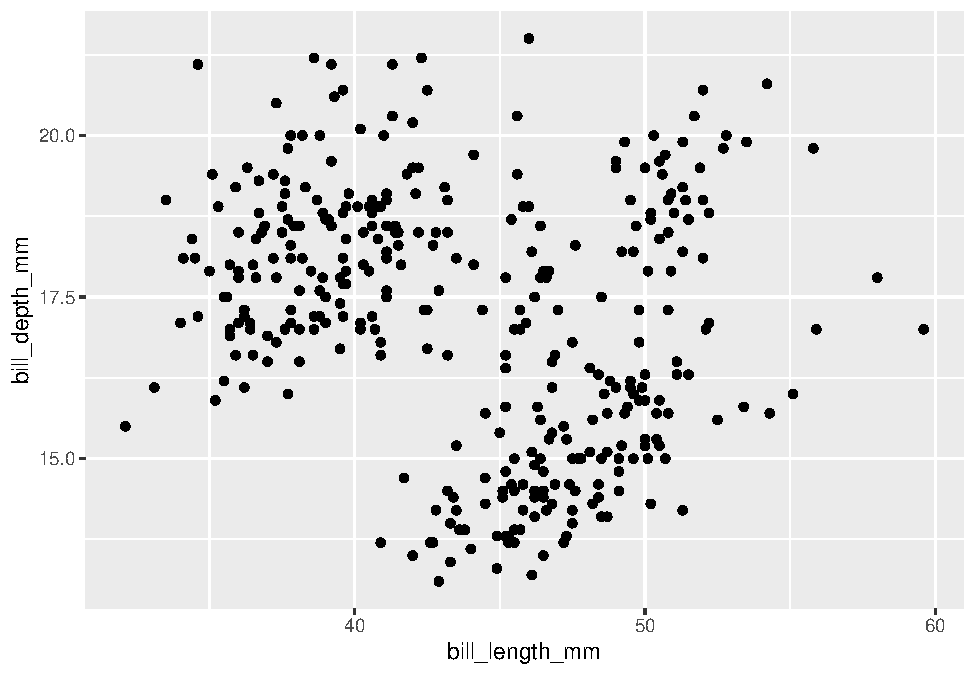
\includegraphics{likert_files/figure-latex/unnamed-chunk-6-1.pdf} Lot of
NAs\ldots{}

Let's check some variables

\begin{Shaded}
\begin{Highlighting}[]
\KeywordTok{table}\NormalTok{(df}\OperatorTok{$}\NormalTok{Gender)}
\end{Highlighting}
\end{Shaded}

\begin{verbatim}
## 
##   Man Woman 
##    43     9
\end{verbatim}

\begin{Shaded}
\begin{Highlighting}[]
\KeywordTok{table}\NormalTok{(df}\OperatorTok{$}\StringTok{`}\DataTypeTok{Power position}\StringTok{`}\NormalTok{)}
\end{Highlighting}
\end{Shaded}

\begin{verbatim}
## 
## Government  Oposition 
##         61         39
\end{verbatim}

\begin{Shaded}
\begin{Highlighting}[]
\KeywordTok{table}\NormalTok{(df}\OperatorTok{$}\NormalTok{Gender, df}\OperatorTok{$}\StringTok{`}\DataTypeTok{Power position}\StringTok{`}\NormalTok{)}
\end{Highlighting}
\end{Shaded}

\begin{verbatim}
##        
##         Government Oposition
##   Man           30        13
##   Woman          5         4
\end{verbatim}

Seems to me that the data are divided in

\emph{demographic data}

{[}1{]} ``RespondentID'' ``Power position'' ``Participation'' ``Year''
``Gender''\\
{[}6{]} ``Language'' ``Parties'' ``YearsMP'' ``Chairman''
``Specialisation''\\
{[}11{]} ``8.LETA/BNS''

\emph{Some questions about use of social media}

``Monitoring'' ``Oft\_radio\_TV'' ``Oft\_newspaper''
``Oft\_publication''\\
{[}16{]} ``FB'' ``draugiem.lv'' ``Instagram'' ``vkontakte''
``Odnoklassniki''\\
{[}21{]} ``Twitter'' ``dont\_use''

\emph{some perceptions about their utility}

the rest of the columns

We can use an special package to create summary table ready for
publication, it's called gtsummary

\begin{Shaded}
\begin{Highlighting}[]
\NormalTok{pacman}\OperatorTok{::}\KeywordTok{p_load}\NormalTok{(gtsummary)}
\end{Highlighting}
\end{Shaded}

Learn about the package here:
\url{https://github.com/ddsjoberg/gtsummary}

For example, a table of the demographic data by power position would be:

\begin{Shaded}
\begin{Highlighting}[]
\NormalTok{df }\OperatorTok\StringTok{ }
\StringTok{  }\KeywordTok{select}\NormalTok{(}\StringTok{`}\DataTypeTok{Power position}\StringTok{`}\OperatorTok{:}\NormalTok{Specialisation) }\OperatorTok\StringTok{  }\CommentTok{# here I select the desired columns to summarize}
\StringTok{  }\NormalTok{gtsummary}\OperatorTok{::}\KeywordTok{tbl_summary}\NormalTok{(}\DataTypeTok{by =} \StringTok{`}\DataTypeTok{Power position}\StringTok{`}\NormalTok{)}
\end{Highlighting}
\end{Shaded}

\begin{longtable}[]{@{}lll@{}}
\toprule
\begin{minipage}[b]{0.57\columnwidth}\raggedright
\textbf{Characteristic}\strut
\end{minipage} & \begin{minipage}[b]{0.18\columnwidth}\raggedright
\textbf{Government}, N = 61\strut
\end{minipage} & \begin{minipage}[b]{0.17\columnwidth}\raggedright
\textbf{Oposition}, N = 39\strut
\end{minipage}\tabularnewline
\midrule
\endhead
\begin{minipage}[t]{0.57\columnwidth}\raggedright
Participation\strut
\end{minipage} & \begin{minipage}[t]{0.18\columnwidth}\raggedright
\strut
\end{minipage} & \begin{minipage}[t]{0.17\columnwidth}\raggedright
\strut
\end{minipage}\tabularnewline
\begin{minipage}[t]{0.57\columnwidth}\raggedright
No\strut
\end{minipage} & \begin{minipage}[t]{0.18\columnwidth}\raggedright
26 (43\%)\strut
\end{minipage} & \begin{minipage}[t]{0.17\columnwidth}\raggedright
22 (56\%)\strut
\end{minipage}\tabularnewline
\begin{minipage}[t]{0.57\columnwidth}\raggedright
yes\strut
\end{minipage} & \begin{minipage}[t]{0.18\columnwidth}\raggedright
0 (0\%)\strut
\end{minipage} & \begin{minipage}[t]{0.17\columnwidth}\raggedright
17 (44\%)\strut
\end{minipage}\tabularnewline
\begin{minipage}[t]{0.57\columnwidth}\raggedright
Yes\strut
\end{minipage} & \begin{minipage}[t]{0.18\columnwidth}\raggedright
35 (57\%)\strut
\end{minipage} & \begin{minipage}[t]{0.17\columnwidth}\raggedright
0 (0\%)\strut
\end{minipage}\tabularnewline
\begin{minipage}[t]{0.57\columnwidth}\raggedright
Year\strut
\end{minipage} & \begin{minipage}[t]{0.18\columnwidth}\raggedright
1,963 (1,954, 1,971)\strut
\end{minipage} & \begin{minipage}[t]{0.17\columnwidth}\raggedright
1,964 (1,956, 1,973)\strut
\end{minipage}\tabularnewline
\begin{minipage}[t]{0.57\columnwidth}\raggedright
Unknown\strut
\end{minipage} & \begin{minipage}[t]{0.18\columnwidth}\raggedright
26\strut
\end{minipage} & \begin{minipage}[t]{0.17\columnwidth}\raggedright
22\strut
\end{minipage}\tabularnewline
\begin{minipage}[t]{0.57\columnwidth}\raggedright
Gender\strut
\end{minipage} & \begin{minipage}[t]{0.18\columnwidth}\raggedright
\strut
\end{minipage} & \begin{minipage}[t]{0.17\columnwidth}\raggedright
\strut
\end{minipage}\tabularnewline
\begin{minipage}[t]{0.57\columnwidth}\raggedright
Man\strut
\end{minipage} & \begin{minipage}[t]{0.18\columnwidth}\raggedright
30 (86\%)\strut
\end{minipage} & \begin{minipage}[t]{0.17\columnwidth}\raggedright
13 (76\%)\strut
\end{minipage}\tabularnewline
\begin{minipage}[t]{0.57\columnwidth}\raggedright
Woman\strut
\end{minipage} & \begin{minipage}[t]{0.18\columnwidth}\raggedright
5 (14\%)\strut
\end{minipage} & \begin{minipage}[t]{0.17\columnwidth}\raggedright
4 (24\%)\strut
\end{minipage}\tabularnewline
\begin{minipage}[t]{0.57\columnwidth}\raggedright
Unknown\strut
\end{minipage} & \begin{minipage}[t]{0.18\columnwidth}\raggedright
26\strut
\end{minipage} & \begin{minipage}[t]{0.17\columnwidth}\raggedright
22\strut
\end{minipage}\tabularnewline
\begin{minipage}[t]{0.57\columnwidth}\raggedright
Language\strut
\end{minipage} & \begin{minipage}[t]{0.18\columnwidth}\raggedright
\strut
\end{minipage} & \begin{minipage}[t]{0.17\columnwidth}\raggedright
\strut
\end{minipage}\tabularnewline
\begin{minipage}[t]{0.57\columnwidth}\raggedright
Latvian\strut
\end{minipage} & \begin{minipage}[t]{0.18\columnwidth}\raggedright
32 (91\%)\strut
\end{minipage} & \begin{minipage}[t]{0.17\columnwidth}\raggedright
11 (65\%)\strut
\end{minipage}\tabularnewline
\begin{minipage}[t]{0.57\columnwidth}\raggedright
Russian\strut
\end{minipage} & \begin{minipage}[t]{0.18\columnwidth}\raggedright
3 (8.6\%)\strut
\end{minipage} & \begin{minipage}[t]{0.17\columnwidth}\raggedright
6 (35\%)\strut
\end{minipage}\tabularnewline
\begin{minipage}[t]{0.57\columnwidth}\raggedright
Unknown\strut
\end{minipage} & \begin{minipage}[t]{0.18\columnwidth}\raggedright
26\strut
\end{minipage} & \begin{minipage}[t]{0.17\columnwidth}\raggedright
22\strut
\end{minipage}\tabularnewline
\begin{minipage}[t]{0.57\columnwidth}\raggedright
Parties\strut
\end{minipage} & \begin{minipage}[t]{0.18\columnwidth}\raggedright
\strut
\end{minipage} & \begin{minipage}[t]{0.17\columnwidth}\raggedright
\strut
\end{minipage}\tabularnewline
\begin{minipage}[t]{0.57\columnwidth}\raggedright
Frakcij? ``No sirds Latvijai''\strut
\end{minipage} & \begin{minipage}[t]{0.18\columnwidth}\raggedright
0 (0\%)\strut
\end{minipage} & \begin{minipage}[t]{0.17\columnwidth}\raggedright
7 (18\%)\strut
\end{minipage}\tabularnewline
\begin{minipage}[t]{0.57\columnwidth}\raggedright
Frakcij? ``Saska?a''\strut
\end{minipage} & \begin{minipage}[t]{0.18\columnwidth}\raggedright
0 (0\%)\strut
\end{minipage} & \begin{minipage}[t]{0.17\columnwidth}\raggedright
24 (62\%)\strut
\end{minipage}\tabularnewline
\begin{minipage}[t]{0.57\columnwidth}\raggedright
Frakcij?��Vienot?ba"\strut
\end{minipage} & \begin{minipage}[t]{0.18\columnwidth}\raggedright
23 (38\%)\strut
\end{minipage} & \begin{minipage}[t]{0.17\columnwidth}\raggedright
0 (0\%)\strut
\end{minipage}\tabularnewline
\begin{minipage}[t]{0.57\columnwidth}\raggedright
Latvijas Re?ionu apvien?bas frakcij?\strut
\end{minipage} & \begin{minipage}[t]{0.18\columnwidth}\raggedright
0 (0\%)\strut
\end{minipage} & \begin{minipage}[t]{0.17\columnwidth}\raggedright
7 (18\%)\strut
\end{minipage}\tabularnewline
\begin{minipage}[t]{0.57\columnwidth}\raggedright
Nacion?l? apvien?bas �Visu Latvijai!�-�T?vzemei un
Br?v?bai/LNNK�frakcij?\strut
\end{minipage} & \begin{minipage}[t]{0.18\columnwidth}\raggedright
17 (28\%)\strut
\end{minipage} & \begin{minipage}[t]{0.17\columnwidth}\raggedright
0 (0\%)\strut
\end{minipage}\tabularnewline
\begin{minipage}[t]{0.57\columnwidth}\raggedright
Pie frakcij?m nepiedero�s deput?ts\strut
\end{minipage} & \begin{minipage}[t]{0.18\columnwidth}\raggedright
0 (0\%)\strut
\end{minipage} & \begin{minipage}[t]{0.17\columnwidth}\raggedright
1 (2.6\%)\strut
\end{minipage}\tabularnewline
\begin{minipage}[t]{0.57\columnwidth}\raggedright
Za?o un Zemnieku savien?bas frakcij?\strut
\end{minipage} & \begin{minipage}[t]{0.18\columnwidth}\raggedright
21 (34\%)\strut
\end{minipage} & \begin{minipage}[t]{0.17\columnwidth}\raggedright
0 (0\%)\strut
\end{minipage}\tabularnewline
\begin{minipage}[t]{0.57\columnwidth}\raggedright
YearsMP\strut
\end{minipage} & \begin{minipage}[t]{0.18\columnwidth}\raggedright
6 (4, 6)\strut
\end{minipage} & \begin{minipage}[t]{0.17\columnwidth}\raggedright
7 (3, 18)\strut
\end{minipage}\tabularnewline
\begin{minipage}[t]{0.57\columnwidth}\raggedright
Unknown\strut
\end{minipage} & \begin{minipage}[t]{0.18\columnwidth}\raggedright
26\strut
\end{minipage} & \begin{minipage}[t]{0.17\columnwidth}\raggedright
22\strut
\end{minipage}\tabularnewline
\begin{minipage}[t]{0.57\columnwidth}\raggedright
Chairman\strut
\end{minipage} & \begin{minipage}[t]{0.18\columnwidth}\raggedright
14 (40\%)\strut
\end{minipage} & \begin{minipage}[t]{0.17\columnwidth}\raggedright
3 (18\%)\strut
\end{minipage}\tabularnewline
\begin{minipage}[t]{0.57\columnwidth}\raggedright
Unknown\strut
\end{minipage} & \begin{minipage}[t]{0.18\columnwidth}\raggedright
26\strut
\end{minipage} & \begin{minipage}[t]{0.17\columnwidth}\raggedright
22\strut
\end{minipage}\tabularnewline
\begin{minipage}[t]{0.57\columnwidth}\raggedright
Specialisation\strut
\end{minipage} & \begin{minipage}[t]{0.18\columnwidth}\raggedright
\strut
\end{minipage} & \begin{minipage}[t]{0.17\columnwidth}\raggedright
\strut
\end{minipage}\tabularnewline
\begin{minipage}[t]{0.57\columnwidth}\raggedright
more than two\strut
\end{minipage} & \begin{minipage}[t]{0.18\columnwidth}\raggedright
25 (71\%)\strut
\end{minipage} & \begin{minipage}[t]{0.17\columnwidth}\raggedright
11 (65\%)\strut
\end{minipage}\tabularnewline
\begin{minipage}[t]{0.57\columnwidth}\raggedright
one or two\strut
\end{minipage} & \begin{minipage}[t]{0.18\columnwidth}\raggedright
10 (29\%)\strut
\end{minipage} & \begin{minipage}[t]{0.17\columnwidth}\raggedright
6 (35\%)\strut
\end{minipage}\tabularnewline
\begin{minipage}[t]{0.57\columnwidth}\raggedright
Unknown\strut
\end{minipage} & \begin{minipage}[t]{0.18\columnwidth}\raggedright
26\strut
\end{minipage} & \begin{minipage}[t]{0.17\columnwidth}\raggedright
22\strut
\end{minipage}\tabularnewline
\bottomrule
\end{longtable}

As you can see, there is \emph{a lot} of data to clean here.

I \emph{strongly suggest} you to learn two of the tidyverse packages:

\url{https://stringr.tidyverse.org/}

\url{https://forcats.tidyverse.org/}

\hypertarget{questions}{%
\section{Questions}\label{questions}}

What are MPs perception on media power compared to other actors (Columns
Agenda\_TV\_radio and Agenda\_written\_press compared to Agenda\_prime;
Agenda\_ministers; Agenda\_MP; Agenda\_parties;
Agenda\_interest\_groups). The survey was in Likert scale 1 - 5);

I don't have much experience with this, so I google:
\url{https://www.google.com/search?q=lickert+data+r\&oq=lickert+data+r\&aqs=chrome}..69i57.7470j0j1\&sourceid=chrome\&ie=UTF-8

I will subset the dataset, selecting some columns only

\begin{Shaded}
\begin{Highlighting}[]
\NormalTok{mydf <-}\StringTok{ }\NormalTok{df }\OperatorTok\StringTok{ }
\StringTok{  }\KeywordTok{select}\NormalTok{(Journalists_indep}\OperatorTok{:}\NormalTok{Agenda_written_press)}
\end{Highlighting}
\end{Shaded}

after googling some \emph{hours} found some packages that can help to
analyze Likert data

\begin{Shaded}
\begin{Highlighting}[]
\NormalTok{sjPlot}\OperatorTok{::}\KeywordTok{plot_likert}\NormalTok{(mydf)}
\end{Highlighting}
\end{Shaded}

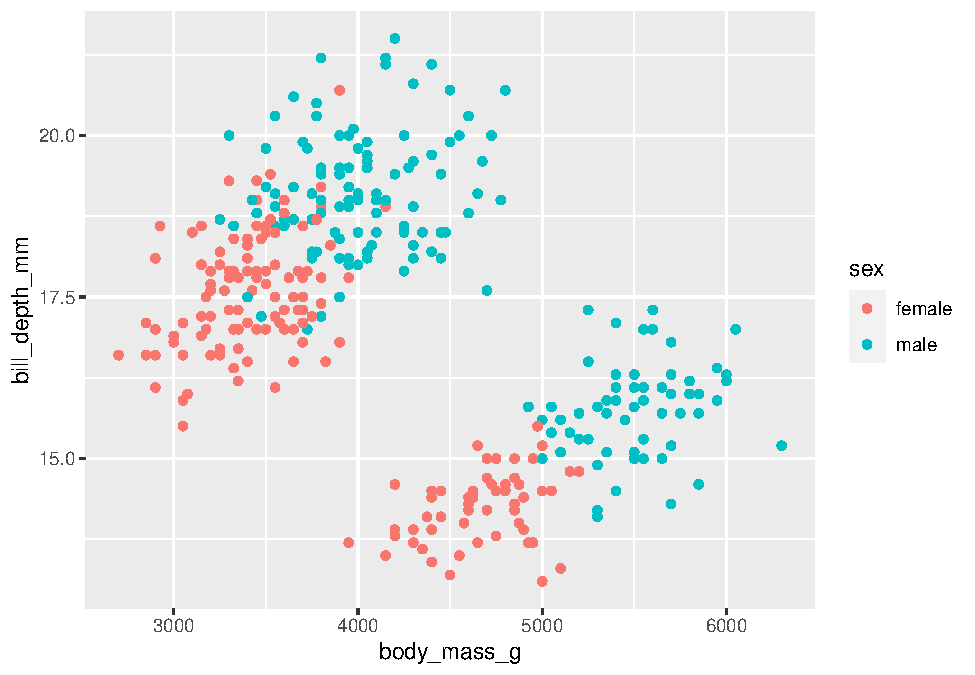
\includegraphics{likert_files/figure-latex/unnamed-chunk-13-1.pdf}

Now ordered

\begin{Shaded}
\begin{Highlighting}[]
\NormalTok{sjPlot}\OperatorTok{::}\KeywordTok{plot_likert}\NormalTok{(}
\NormalTok{  mydf,}
  \DataTypeTok{grid.range =} \KeywordTok{c}\NormalTok{(}\FloatTok{1.2}\NormalTok{, }\FloatTok{1.4}\NormalTok{),}
  \DataTypeTok{expand.grid =} \OtherTok{FALSE}\NormalTok{,}
  \DataTypeTok{values =} \StringTok{"sum.outside"}\NormalTok{,}
  \DataTypeTok{show.prc.sign =} \OtherTok{TRUE}
\NormalTok{)}
\end{Highlighting}
\end{Shaded}

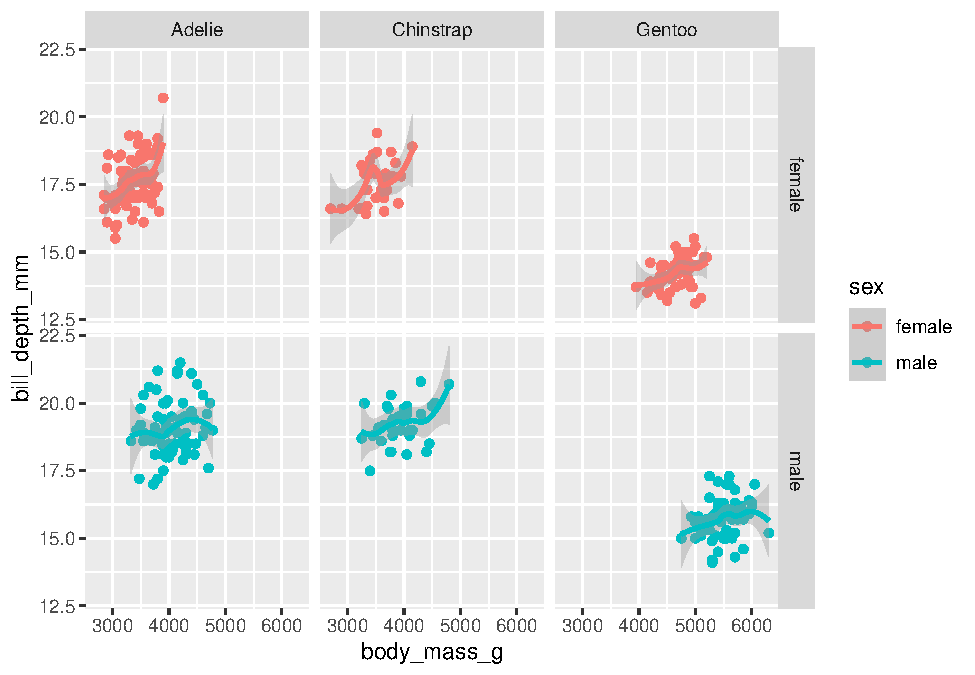
\includegraphics{likert_files/figure-latex/unnamed-chunk-14-1.pdf}

\hypertarget{learn-more}{%
\section{Learn more}\label{learn-more}}

learn about the sjPlot package here:

\url{https://strengejacke.github.io/sjPlot/}

\hypertarget{learn-even-more}{%
\section{Learn even more!}\label{learn-even-more}}

Check the survey package, specially designed to analyze data from
surveys

\url{http://r-survey.r-forge.r-project.org/survey/}

since is quite an old package, there is a tool that allows you to work
with dplyr from tidyverse package:

\url{https://github.com/gergness/srvyr}

\end{document}
